
\vspace{-0.2cm}
\section{Effects of {\color{cc2}data distribution  \texorpdfstring{$p_{\textrm{data}}$}{TEXT}} on attention sink}
\vspace{-0.2cm}
\label{sec5}

\begin{figure}[t]
\centering
% \vspace{-0.2cm}
\begin{subfigure}[t]{\textwidth}
    \centering
    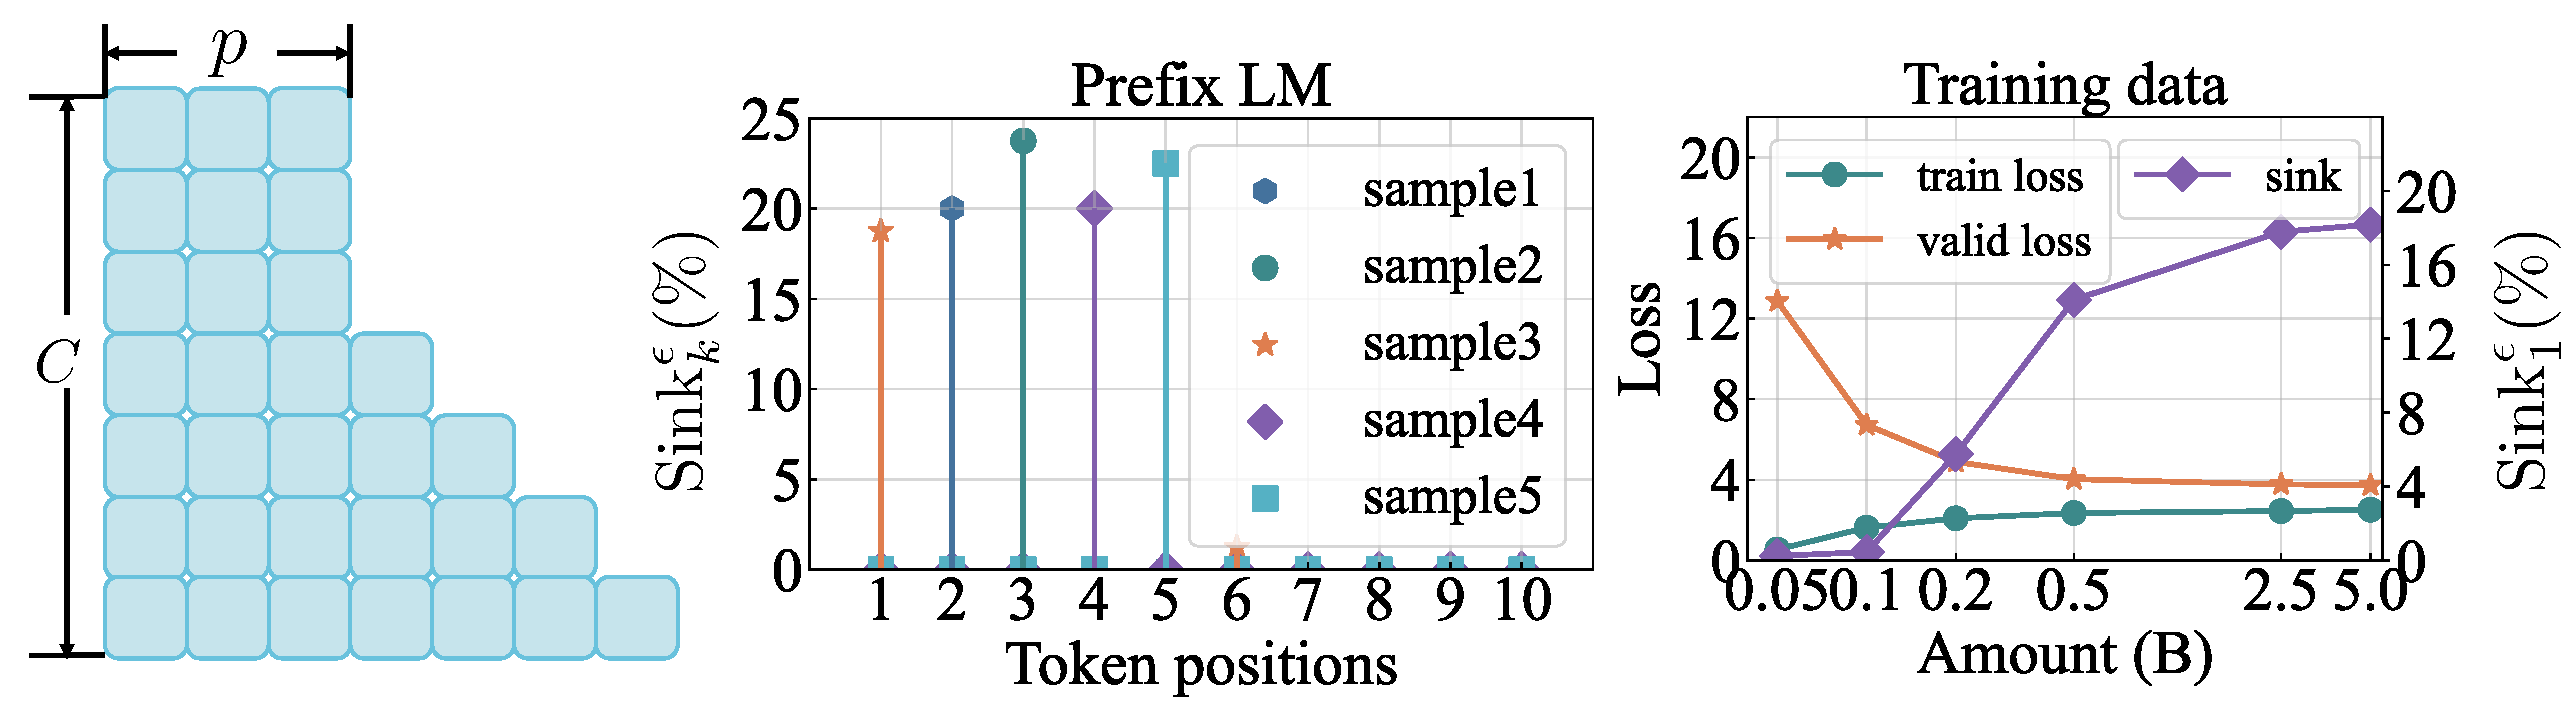
\includegraphics[width=\textwidth]{figures/data_prefix.pdf}
\end{subfigure}
\vspace{-0.65cm}
\caption{(\emph{Left}) Attention pattern for prefix language modeling. (\emph{Middle}) Attention sink does not only appear on the first token but among the prefix tokens for LMs with $p=\textrm{5}$. (\textit{Right}) With less training data, attention sink disappears. Meanwhile, trained LMs demonstrate overfitting behaviors.\looseness=-1}
\vspace{-0.15cm}
\label{data}
\end{figure}

\textbf{Training data amount.} In the default setup, we consider 5B tokens. We wonder whether the attention sink emerges if we further constrain the data within a fixed compute budget. Therefore, we constrain the training data to 5B, 2.5B, 500M, 200M, 100M, and 50M. Meanwhile, we fix the batch size and optimization steps. As visualized in Figure~\ref{data}(\emph{Right}), with less training data, attention sink disappears. Further evidence in Figure~\ref{appendix_overfit} shows that this is not related to overfitting.\looseness=-1

\textbf{Randomness in data distribution.} After packing documents into chunks, we re-sample the first token within the chunk $\boldsymbol{x}_1\sim \textrm{Uniform}(\mathbb{V})$. The trained LM has the metric $\textrm{Sink}_1^\epsilon=\textrm{27.03\%}$, even larger than the default setup. This further validates the low semantic information of the sink token. We also consider $\boldsymbol{x}_1\textrm{,}\,\boldsymbol{x}_2\sim \textrm{Uniform}(\mathbb{V})$, and we find attention sink shifts to the second token with $\textrm{Sink}_2^\epsilon=\textrm{14.08\%}$ while the attention sink on the first token is much less obvious $\textrm{Sink}_1^\epsilon=\textrm{1.98\%}$. But when only sample $\boldsymbol{x}_2\sim \textrm{Uniform}(\mathbb{V})$, the attention sink still always appears on the first token ($\textrm{Sink}_1^\epsilon=\textrm{20.99\%}$). Additionally, we find with more random tokens during pre-training, attention sink tends to disappear.\looseness=-1

\textbf{Fixing token in a specific position.} \citet{xiao2023efficient} considered a learnable token in the first token position within each chunk, which can be considered as $\boldsymbol{x}_1\sim \mathbb{I}(\boldsymbol{x}=\boldsymbol{x}_{\textrm{fix}})$. We also consider fixing the token $\boldsymbol{x}_{\textrm{fix}}$ in the second/third token position during pre-training. Consequently, the attention sink always appears in the fixed token instead of the first token, as shown in Table~\ref{batch_fix}(\emph{Right}).

\vspace{-0.1cm}
\begin{abox} % are we tired of takeaway boxes? :>
    \looseness -1 \textbf{Takeaways:} 1.~Attention sink emerges after LMs are trained on sufficient training data. 2.~Attention sink could be shifted to other positions rather than the first token if modifying $\color{cc2} p_{\textrm{data}}$.\looseness=-1% at test time.
\end{abox}

% \begin{figure}[t]
% \centering
% \begin{subfigure}[t]{0.48\textwidth}
%     \centering
%     \includegraphics[width=\textwidth]{figures/tinyllama_data.pdf}
% \end{subfigure}
% % \subfigure[]{\includegraphics[width=0.45\textwidth]{figures/domains_metric1.pdf}}
% % \begin{subfigure}[htbp]{0.48\textwidth}
% %     \centering
% %     \includegraphics[width=\textwidth]{figures/tinyllama_sink.pdf}
% % \end{subfigure}
% \hfill
% % \begin{subfigure}[htbp]{0.48\textwidth}
% %     \centering
% %     \includegraphics[width=\textwidth]{figures/tinyllama_loss.pdf}
% % \end{subfigure}
% \vspace{-0.3cm}
% \caption{(\textit{Left}) Dynamics of attention sink amplitude in each block during the training (\textit{Right}) Loss dynamics during the training in the default setup.
% }
% \label{data}
% \end{figure}


% \begin{table}[htbp]
% \begin{center}
% \begin{tabular}{l|cccccc}
% \toprule
% Training data & 5B & 2.5B & 500M & 200M & 100M & 50M \\
% \midrule
% $\textrm{Sink}_1^{\epsilon}$(\%) & 18.18 & 17.79 & 14.11 & 5.74 & 0.45 & 0.24 \\
% Valid loss & 3.73 & 3.77 & 4.03 & 4.89 & 6.72 & 12.87 \\
% \bottomrule
% \end{tabular}
% \end{center}
% \vspace{-.2cm}
% \caption{Data diversity.}
% \vspace{-.2cm}
% \label{data}
% \end{table}


% \subsection{BOS Tokens}


